%\section{Outline}
%\input{includes/thesis}
%Given a $m \times n$ system of equations: 
%\section*{Define arithmetic operations ($+, -, \times$) on matrices}
% \section*{Introduction}


%\subsubsection*{Objectives}
%\begin{itemize}
%	\item Calculate length of a vector
%	\item Calculate dot products
%	\item Use dot product to determine  
%\end{itemize}



\subsubsection*{Learning outcomes}
Be able to:
\begin{itemize}
	\item Represent a system of linear equations as a matrix equation
	 \item Solve system of linear equations
	 % \item Write the identity matrix
	 \item View solutions from a geometric viewpoint
	 \item Understand $A{\bf x}$ as a linear combination of columns of $A$
	 \item Identify software used in linear algebra
	
\end{itemize}





\rule[0.01in]{\textwidth}{0.0025in}
% ---------------------------------------------------- % 




A \textbf{linear equation} in $n$ variables (or unknowns) is an equation of the form
\[ a_1 x_1 + a_2 x_2 + a_3 x_3 + \dots + a_n x_n = b \]

where $a_1, a_2, \dots, a_n$ and $b$ are real numbers and $x_1, x_2, \dots, x_n$ are variables. 
 

 \begin{tcolorbox}[colback=yellow!10!,colframe=gray!15!]

A \textbf{linear system} of $m$ equations in $n$ unknowns is then a system of the form
\[ 
\begin{cases} 
a_{11} x_1 + a_{12} x_2 + a_{13} x_3 + \dots + a_{1n} x_n &= y_1\\
 a_{21} x_1 + a_{22} x_2 + a_{23} x_3 + \dots + a_{2n} x_n &= y_2\\
a_{31} x_1 + a_{32} x_2 + a_{33} x_3 + \dots + a_{3n} x_n &= y_3\\

\vdots      &\vdots \\

a_{m1} x_1 + a_{m2} x_2 + a_{m3} x_3 + \dots + a_{mn} x_n &= y_m
\end{cases}
 \]
 \end{tcolorbox} 


The coefficients on the left-side of the system can be extracted and represented with a matrix, 

\[ 
A =  \begin{bmatrix} 
	a_{11} & a_{12} & a_{13}	& \cdots & a_{1n} \\
 	a_{21} & a_{22} & a_{13}	& \cdots & a_{2n} \\
  	a_{31} & a_{32} & a_{33}	& \cdots & a_{3n} \\
	\vdots 	&	&	& \ddots & \vdots \\
    	a_{m1} & a_{m2} & a_{m3}	& \cdots & a_{mn} \\
    \end{bmatrix}  
 \]


The vector of unknowns is, 
\[ 
{\bf x} = \begin{bmatrix} x_1 \\ x_2 \\ \vdots \\ x_n \end{bmatrix}
\]



The coefficients on the right-side can be represented with a vector, 
\[ 
{\bf y} = \begin{bmatrix} y_1 \\ y_2 \\ \vdots \\ y_m \end{bmatrix}
\]



\subsubsection*{Matrix Equation}
The linear equations can be represent by a matrix equation.

\begin{align*}  
A {\bf x} &= {\bf y}\\
 \begin{bmatrix} 
	a_{11} & a_{12} & a_{13}	& \cdots & a_{1n} \\
 	a_{21} & a_{22} & a_{23}	& \cdots & a_{2n} \\
  	a_{31} & a_{32} & a_{33}	& \cdots & a_{3n} \\
	\vdots 	&	&	& \ddots & \vdots \\
    	a_{m1} & a_{m2} & a_{m3}	& \cdots & a_{mn} \\
    \end{bmatrix}  \begin{bmatrix} x_1 \\ x_2 \\ \vdots \\ x_n \end{bmatrix} &= \begin{bmatrix} y_1 \\ y_2 \\ \vdots \\ y_m \end{bmatrix} 
   \end{align*}


\subsubsection*{Linear Combination Equation}
The linear equations can also be represent  by the linear combination: 
\[ x_1 \begin{bmatrix} a_{11} \\ a_{21} \\ \vdots \\ a_{m1} \end{bmatrix} + x_2  \begin{bmatrix} a_{12} \\ a_{22} \\ \vdots \\ a_{m2} \end{bmatrix} + \cdots + x_n  \begin{bmatrix} a_{1n} \\ a_{2n} \\ \vdots \\ a_{mn} \end{bmatrix} = \begin{bmatrix} y_1 \\ y_2 \\ \vdots \\ y_m \end{bmatrix}
\]

% ---------------------------------------------------- % 
\rule[0.01in]{\textwidth}{0.0025in}
% ---------------------------------------------------- % 

 





\textbf{There are 3 possibilities for solutions of a system of equations}:
\begin{enumerate}
	\item One Solution
	\item No solution (0 solutions)
	\item Infinite Solutions
\end{enumerate}


% ---------------------------------------------------- % 
\rule[0.01in]{\textwidth}{0.0025in}
% ---------------------------------------------------- % 

\begin{definition} (\textbf{Consistent System}) -  A system that has at least one solution, (i.e., nonempty solution set).  \end{definition}






 
\begin{definition} (\textbf{Inconsistent System}) -  A system that has no solution, solution set is empty.  \end{definition}



% ---------------------------------------------------- % 
\rule[0.01in]{\textwidth}{0.0025in}
% ---------------------------------------------------- % 





In two-dimensions, the graphical view a the three possibilities are displayed in Figure \ref{fig:system1}. 

%  \includegraphics[width=6in]{Figures/3possiblities.png} 

\begin{figure}[h!]
\centering
\begin{subfigure}{.33\textwidth}
  \centering

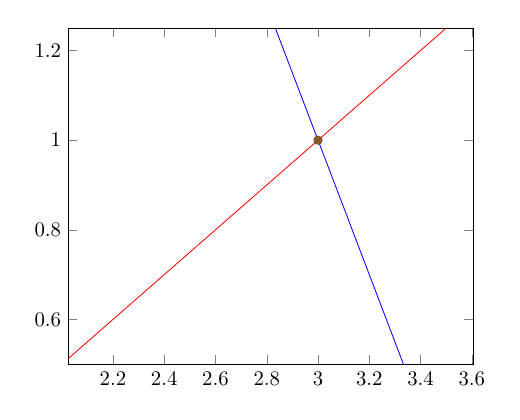
\begin{tikzpicture}[scale=0.75] \begin{axis}[ymin=0.5,
	ymax=1.25,
]
    % density of Normal distribution:
    \addplot [
        red,
        domain=-1:4,
        samples=20
    ]
        {0.5*x-0.5};
\addplot [
        blue,
        domain=-1:5,
        samples=20
    ]{-1.5*x+5.5};

\addplot coordinates {
(3,1)
};

\end{axis}
\end{tikzpicture}
  \caption{One Solution}
  \label{fig:subs1}
\end{subfigure}%
\begin{subfigure}{.33\textwidth}
  \centering

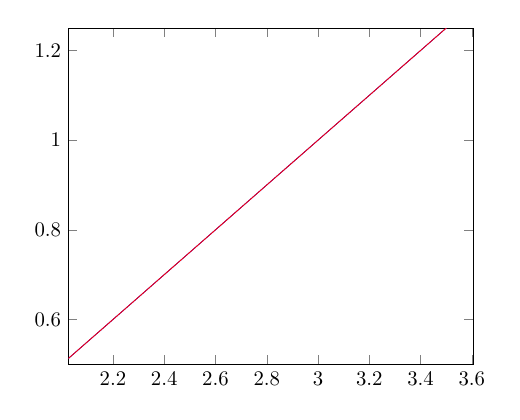
\begin{tikzpicture}[scale=0.75] \begin{axis}[ymin=0.5,
	ymax=1.25,
]
    % density of Normal distribution:
    \addplot [
        blue,
        domain=-1:4,
        samples=20
    ]
        {0.5*x-0.5};
\addplot [
        red,
        domain=-1:5,
        samples=20
    ]{0.5*x-0.5};
\end{axis}
\end{tikzpicture}

  \caption{Infinite Solutions (same line)}
  \label{fig:subs2}
\end{subfigure}%
\begin{subfigure}{.33\textwidth}
  \centering

\begin{tikzpicture}[scale=0.75] \begin{axis}[ymin=0.5,
	ymax=1.25,
]
    % density of Normal distribution:
    \addplot [
        red,
        domain=-1:4,
        samples=20
    ]
        {0.5*x-0.5};
\addplot [
        blue,
        domain=-1:5,
        samples=20
    ]{0.5*x+0.5};
\end{axis}
\end{tikzpicture}

  \caption{No Solution (parallel lines)}
  \label{fig:subs3}
\end{subfigure}%
\caption{Possible solutions of a system of equations in two-dimensions}
\label{fig:system1}
\end{figure}






% ---------------------------------------------------- % 
\rule[0.01in]{\textwidth}{0.0025in}
% ---------------------------------------------------- % 









\begin{example}
$ \begin{array}{rcl}& & \\ x_1 - 3x_2 & = & 2 \\ 5x_1 - 2 x_2 & = & 7 \end{array}$

The coefficient matrix of this system is, 
\[  \begin{bmatrix}
1 & -3 \\ 5 & -2 
\end{bmatrix}
\]
\end{example}


\begin{example}
$ \begin{array}{rcl}& & \\ x - 2y & = & 1 \\ 3x + 2 y & = &11 \end{array}$

Two ways to view these equations:


\begin{figure}[h!]
\centering
\begin{subfigure}{.5\textwidth}
  \centering

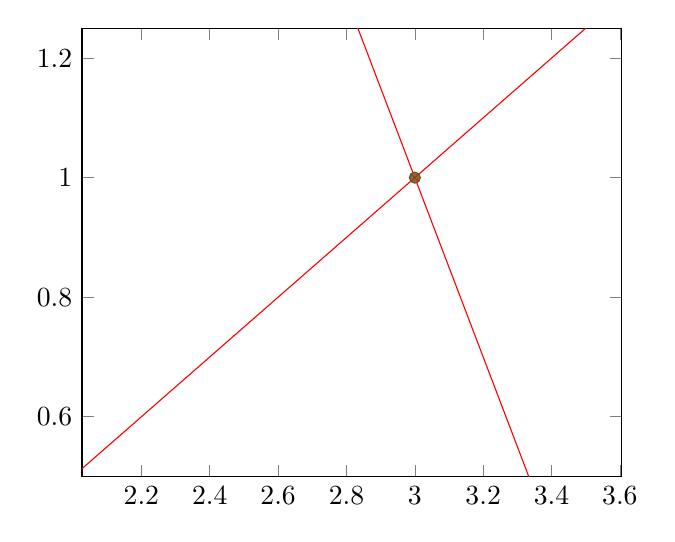
\begin{tikzpicture} \begin{axis}[ymin=0.5,
	ymax=1.25,
]
    % density of Normal distribution:
    \addplot [
        red,
        domain=-1:4,
        samples=20
    ]
        {0.5*x-0.5};
\addplot [
        red,
        domain=-1:5,
        samples=20
    ]{-1.5*x+5.5};

\addplot coordinates {
(3,1)
};

\end{axis}
\end{tikzpicture}

  \caption{Row view}
  \label{fig:sub1}
\end{subfigure}%
\begin{subfigure}{.5\textwidth}
  \centering

   \includegraphics[scale=0.95]{figures/s2_2} 

  \caption{Column view}
  \label{fig:sub2}
\end{subfigure}
\caption{Two views of the solution of a system of equations}
\label{fig:system2}
\end{figure}


\end{example}


% ---------------------------------------------------- % 
%\rule[0.01in]{\textwidth}{0.0025in}
% ---------------------------------------------------- % 

 



%\begin{definition}[Scalar Multiplication] - If $A$ is a matrix and $\alpha \in \mathbb{F}$ (e.g., $\mathbb{F} = \mathbb{R}$), then $\alpha A$ is the $m \times n$ matrix whose $(i,j)$ entry is $\alpha a_{ij}$.
%\end{definition}


%\begin{example}
%Let \[ A = \begin{bmatrix} 2 & 1 & -3 \\ 3 & 5 &1\end{bmatrix} \] and $\alpha =2$, then \[  \alpha A = 2A= \begin{bmatrix} 4 & 2 & -6 \\ 6 & 10 & 2 \end{bmatrix} \] 
%\end{example}


%\textbf{MATLAB commands}
%\begin{verbatim}
%>> A=[2 1 -3;3 5 1]
%>> 2*A
%\end{verbatim}





% ---------------------------------------------------- % 
\rule[0.01in]{\textwidth}{0.0025in}
% ---------------------------------------------------- % 



%
%%
%%%						  
%%%% SECTION:  Software
%%%
%%
%

\subsection*{Software}
Many software perform linear algebra operations.  We will use MATLAB.  A small list of other software include:
\begin{itemize}
	\item Python
	\item Julia
	\item Mathematica
	\item Maple
	\item R
\end{itemize}







\subsection*{In Class Problems\footnote{Not due for homework.}}
\begin{enumerate}
\item Find the matrices that act in special ways on vectors
	\begin{enumerate}
	
		\item Multiply the matrix and vector by writing as a linear combination of the columns and adding.
			\[ \begin{bmatrix} 1 & 2 & 4\\ -2 & 3 & 1 \\ -4 & 1 & 1 \end{bmatrix} \begin{bmatrix} 2 \\ 2  \\3 \end{bmatrix} \]
			
			See problem 9 -- 11.
			
		
		\item $2 \times 2$ identify matrix $I$ such that $I\begin{bmatrix} x \\ y \end{bmatrix} = \begin{bmatrix} x \\ y \end{bmatrix}$
		
		\item $2 \times 2$ exchange matrix $P$ such that $P\begin{bmatrix} x \\ y \end{bmatrix} = \begin{bmatrix} y \\ x \end{bmatrix}$
		
		\item $2 \times 2$ 90 degree rotation matrix $R$ such that $R\begin{bmatrix} x \\ y \end{bmatrix} = \begin{bmatrix} y \\ -x \end{bmatrix}$
		
		\item $2 \times 2$ 180 degree rotation matrix
		
		\item What $2 \times 2$ matrix subtracts the first component from the second component? 
		What $3 \times 3$  does the same? 
		\[ E \begin{bmatrix} x \\ y \end{bmatrix} = \begin{bmatrix} x \\ y-x \end{bmatrix} \]
		\[ E \begin{bmatrix} x \\ y \\ z \end{bmatrix} = \begin{bmatrix} x \\ y-x \\ z \end{bmatrix} \]
	
		
	\end{enumerate}
\end{enumerate}






% ---------------------------------------------------- % 
\rule[0.01in]{\textwidth}{0.0025in}
% ---------------------------------------------------- % 


\subsubsection*{Next time...}
Section 2.2: Gaussian Elimination





\subsubsection*{Homework}
\textsection2.1: \#4, 7, 9, 19, 22









%\begin{tcolorbox}[colback=yellow!10!,colframe=gray!15!]
%\begin{theorem}[Cauchy-Schwarz Inequality]
%If ${\bf x} $ and ${\bf y} $ are vectors (in an inner product space) then
 %\[ |  {\bf x} \cdot {\bf y} | \le ||{\bf x}|| \,  ||{\bf y}|| \]
 %\end{theorem}	 
%\end{tcolorbox} 



